\section{Automatic Pipeline Synthesis}
\begin{figure*}[htb]
\centering
  \begin{subfigure}[t]{0.8\textwidth}
  \centering
  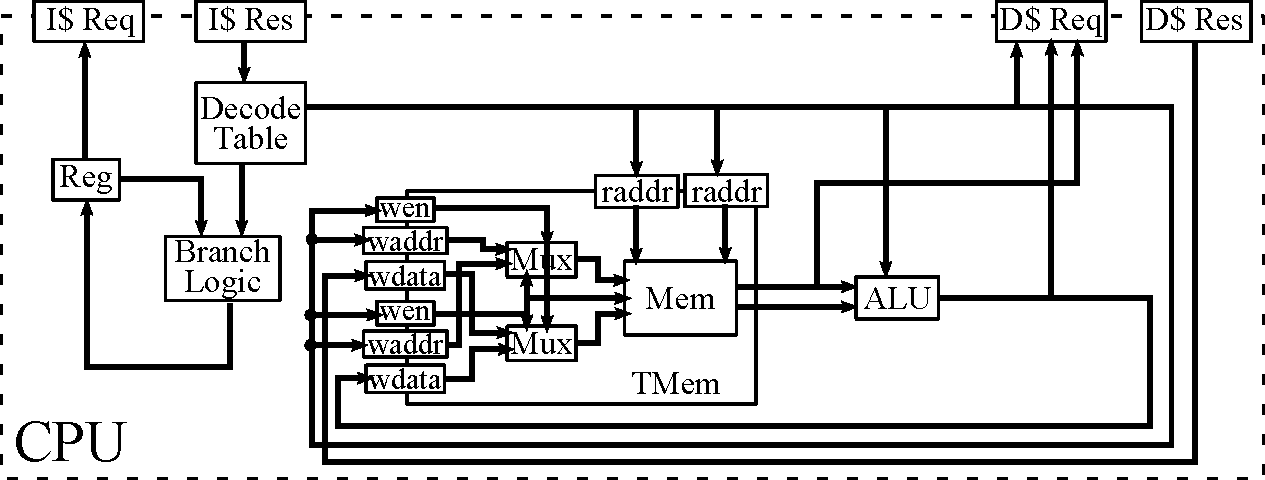
\includegraphics[width=\textwidth]{figures/pipeline.pdf}
  \caption{{\bf Datapath Graph}. CPU datapath represented as a
    directed dataflow graph in Chisel.}
  \label{fig:datapathgrah}
  \end{subfigure}
  \begin{subfigure}[t]{0.8\textwidth}
  \vspace{20pt}
  \centering
  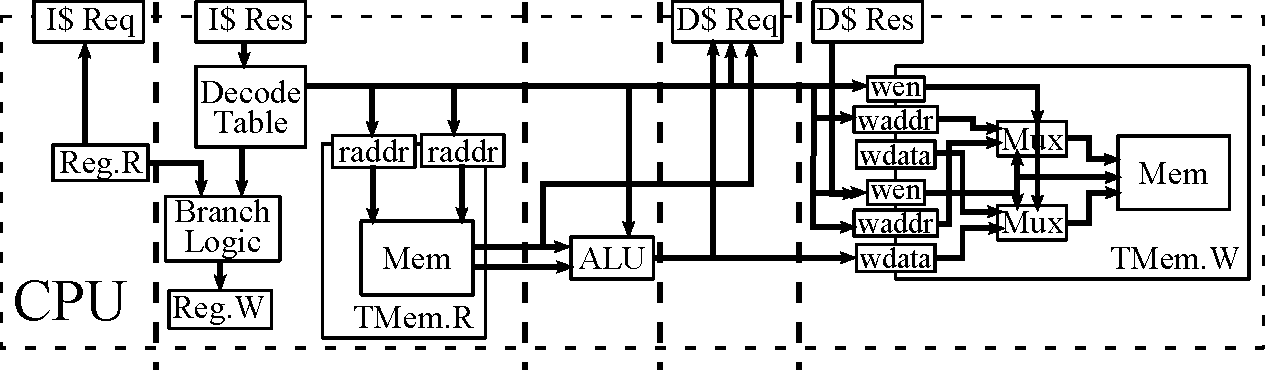
\includegraphics[width=\textwidth]{figures/pipelinedag.pdf}
  \caption{{\bf Datapath DAG}. 5-stage CPU datapath turned into a
    directed acyclic graph by breaking {\tt Reg} nodes and {\tt
      TransactionalMem} into read and write ports. The dashed lines
    represent pipeline boundaries.}
  \label{fig:datapathdag}
  \end{subfigure}
\caption{{\bf 5-stage CPU Datapath}. ALU = arithmetic logic unit. D\$
  = data cache. I\$ =  instruction cache. TMem =
  TransactionalMem. {\tt x}.R = read port of node {\tt x}. {\tt x}.W =
  write port of node {\tt x}}
\label{fig:datapath}
\end{figure*}

There are three major parts to our automatic pipeline synthesis
tool. Given a datapath and a pipeline specification, we first
determine register placement and color every node in the datapath with
their appropriate stage number. Next, we analyze the datapath to find
all sources of hazards and produce a list of hazard
conditions. Finally, we resolve these hazards through either
interlocks (default), speculation, or bypassing.

We perform the Chisel Node graph transformations required for pipeline register placement and hazard resolution through the Chisel's elabortion time interface, which takes in a list of transformations on the Chisel Node graph and executes the transformations at elaboration time.
\subsection{Pipeline Register Placement and Stage Coloring}
The user annotates a set of combinational logic nodes
and architectural state read/write ports with pipeline stage
numbers. The user can annotate just the big pieces of combinational
logic and architectural state they care about, such as ALUs, register
files, or caches, and the automatic synthesis tool will infer the
placement of all the other parts of the datapath. Of course, the user
gains more control over the placement of the pipeline registers by
adding more pipeline stage annotations. The user can have complete
control over the placement of the pipeline registers if they annotate
every combinational logic node and read/write port in the datapath. 

The elaboration time transformation function
first breaks the original cyclic Chisel Node graph into an acyclic
graph by separating architectural states into read ports and write
ports. Then the known pipeline stage numbers from the user annotated
Chisel Nodes are propagated to their producers and consumers in a
pseudo breadth-first-search(BFS) manner. When two propagation
frontiers meet at the same node, propagation down that path stops and
pipeline registers are inserted at that node. We also record the stage
numbers of all Chisel Nodes after the stage propagation and pipeline
register insertion for use in detecting pipeline hazards in the next
stage of the automatic pipeline synthesis. 

{\bf Pipeline Stage Propagation Details}. Nodes and their stage
numbers are kept track of in a map of Nodes to List of Stage Numbers
that we will refer to as the stage number map. Initially, only the
user annotated nodes have non-empty values in the stage number map. In
the pseudo BFS traversal, the propagation frontier(i.e. the nodes that
have yet to propagate out their stage numbers) is kept track of with a
queue. The propagation frontier queue is initialized with the user
annotated nodes. As with a normal BFS traversal, the head of the
propagation frontier queue is dequeued, some visit operation is
performed on the dequeued node, and its children, which includes both
producers and consumers, are enqueued onto the propagation frontier
queue. Unlike a normal BFS traversal, the dequeued node maybe
re-enqueued by the visit operation. In this case, the visit operation
tries to propagate out the stage number of the dequeued node to its
children by appending the dequeued node's stage number to its
children's stage number list in the stage number map if the dequeued
node is not the meeting point of two propagation frontiers. If it is
not currently possible to propagate out the node's stage number, the
visit operation re-enqueues the node onto the propagation frontier
queue for a retry later. The node can propagate out its stage number
if the following conditions are true: (1) the node has exactly one
stage number in its stage number list in the stage number map and (2)
all of the nodes children are ready to receive a stage number.  

Condition (1) makes sure that the propagation front has reached the
node, which means that the node must have at least one stage number in
its stage number list, and that two propagation frontiers have not
meet at that node, which means that the node must have less than 2
stage numbers in its stage number list.  

Condition (2) makes sure that the dequeued node propagates out its
stage number to all of its children in an atomic manner. This is
necessary because the propagation would produce incorrect results if
the node managed to propagate out its stage number to only some of its
children before two propagation frontiers meet at that node and stop
the node from propagating its stage to the rest of its children. The
node can only propagate its stage number to all of its children
atomically if it waits until all of its children are ready and
propagates to all of them at the same time, before the next node
dequeued from the propagation frontier queue. The next paragraph
discusses why some children may not be immediately ready to receive a
stage number propagation. 

We need to check that nodes are ready to receive a stage number
because we need to enforce that a node has a stage number {\tt >=} the
stage numbers of all of its producer nodes and {\tt <=} the stage
numbers for all of its consumer nodes. For nodes with multiple
producers, such as combinational logic nodes, the stage number
propagated to the node from the producer side should be the maximum of
the stage numbers of all of its producers. For nodes with multiple
consumers the stage number propagated to the node from the consumer
side should be minimum of the stage number of all its consumers. Thus,
a node is ready to receive a stage number propagation from its
producer side if a propagation frontier has reached all of its
producer nodes and a node is ready to receive a stage number
propagation from its producer side if a propagation frontier has
reached all of its consumer nodes. 

Once the stage number propagation is complete, we traverse the Chisel
Node graph again and insert the appropriate number of pipeline
registers between any adjacent nodes with different stage numbers and
on any nodes with more than one stage number in its stage numbers list
in the stage numbers map. Refer to Figure~\ref{fig:propagate} for pseudo code on the
stage number propagation algorithm. 

\begin{figure}[htb]
\centering
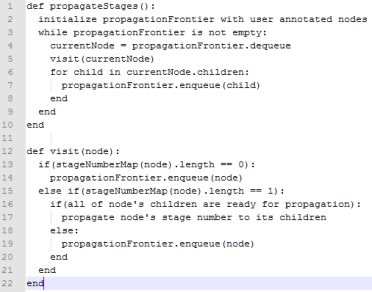
\includegraphics{figures/propagate_pseudo_code.pdf}
\caption{{\bf Pipeline Stage Propagate Pseudo Code}}
\label{fig:propagate}
\end{figure}

\subsection{Hazard Discussion}
\begin{figure*}[htb]
\centering
  \begin{subfigure}[t]{0.8\textwidth}
  \centering
  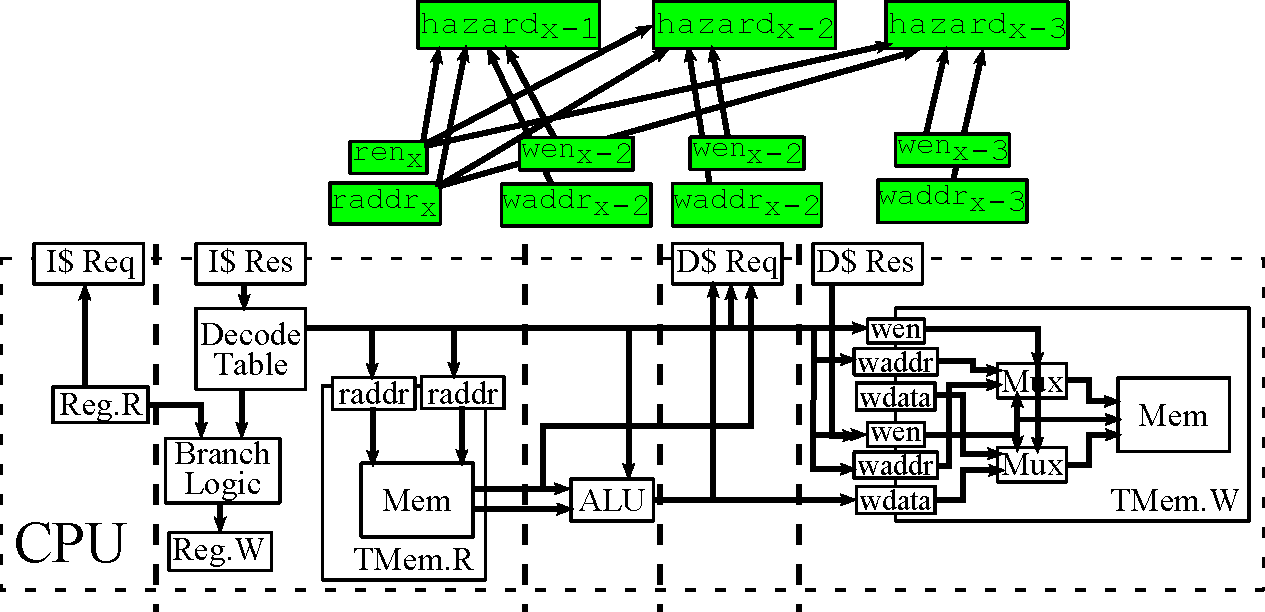
\includegraphics[width=\textwidth]{figures/pipelinehazard.pdf}
  \caption{{\bf Hazard Detection}. All the hazards that
    the {\tt TransactionalMem} generates in a 5-stage pipeline.}
  \label{fig:haz}
  \end{subfigure}
  \begin{subfigure}[t]{0.8\textwidth}
  \vspace{20pt}
  \centering
  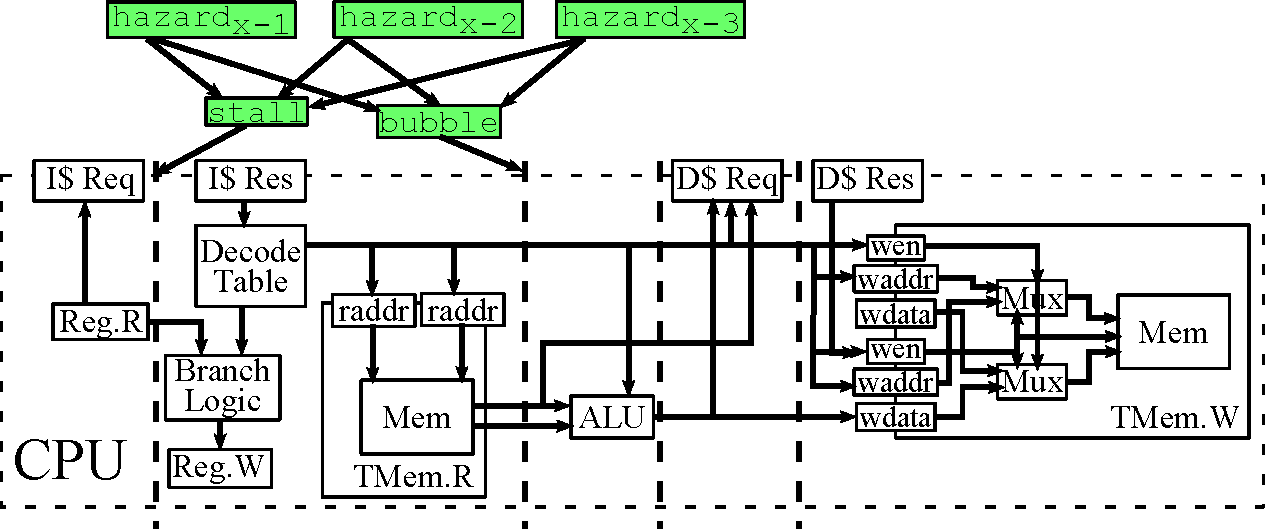
\includegraphics[width=\textwidth]{figures/pipelineinterlock.pdf}
  \caption{{\bf Interlocks}. The hazard conditions stall the
  first and second stage and push bubbles into the third stage.}
  \label{fig:int}
  \end{subfigure}
\caption{Resolving hazards through interlocks.}
\label{fig:hazint}
\end{figure*}

{\bf Hazard Types}. Pipeline hazards fall into the categories of
control hazard, data hazard, and structural hazard. Control hazards
can be viewed as read-after-write(RAW) data hazards on the PC register
in the context of processors. Write-after-read and write-after-write
data hazards are not possible because we enforce that architectural
state elements cannot have write ports be placed in a pipeline stage
before the state element's read ports. Since we don't handle structural
hazards, the only hazard that the automatic synthesis tools have to
handle is RAW data hazards.

RAW data hazards can be resolved in one of three ways: interlocking,
bypassing, and speculation. The default RAW hazard resolution option
is interlocking, so no additional specification is needed if the user
wants to use interlocking to resolve all pipeline hazards.

In order to resolve RAW hazard through speculation, the user annotates
architectural state elements with a speculated write data value. We
give the user freedom to use any Chisel data node for the speculated
write data value, so the user may put in anything for the speculated
value, including output from hand written predictor modules. The
automatic synthesis tools will generate logic that updates the state
element with the speculated value, logic that detects when a
miss-speculation occurs, and recovery logic that writes the actual write
data value into the state element and kills transactions in the
datapath that depend on the speculated value when a miss-speculation
occurs. The automatic synthesis tool does not need to restore
architectural state in state elements other than the state element that
caused the miss-speculation because we enforce that no architectural
state element write ports are placed in pipeline stages where there
maybe an unchecked speculated value. 

In order to resolve RAW hazard through bypassing, the user adds the
read port of an architectural state element to a list of read ports to
be bypassed to and the the automatic synthesis tool will generate logic
that bypasses from all possible bypassing paths to all the consumers
of that read port. The user can also
add write ports of architectural state to a list of write ports to be avoided in the bypassing logic generation. This tells the automatic synthesis tools to never
bypass from the write paths associated with those write ports, which
is desirable when the user knows that a particular write path has a
long critical path.

The pipelining specification is completely separate from the datapath
specification, which allows the user to easily change pipeline
parameters by reusing the datapath specification and changing the
pipelining specification.

{\bf Detection}. Inserting pipeline registers into the datapath
graph introduces pipelining hazards that are not present in the
unpipelined datapath. Here we discuss how to handle data hazards which
result from a transaction reading a state element (a {\tt Reg} node or a
{\tt TransactionalMem}) before an earlier transaction writes to that state
element. 

We first search through the datapath graph to find all state
elements. For every state element, we determine whether or not a
hazard exists on it. If there is a hazard on a state element, we add
the hazard condition into a list. For {\tt Reg} or {\tt TransactionalMem}, a
hazard condition exists if the state element belongs in a stage that precedes the
stage of its write enable or write data signal. The actual Boolean
hazard condition is {\tt wen \&\& ren} for a {\tt Reg} node and
{\tt wen \&\& ren \&\& waddr == raddr} for a {\tt TransactionalMem}.

Figure~\ref{fig:haz} shows the hazard conditions that our tool
identifies on the {\tt TransactionalMem}. when analyzing the generated pipeline in
Figure~\ref{fig:datapathdag}. We first search the pipeline for all
state elements. In this example, the {\tt Reg} node and the 
{\tt TransactionalMem} are the only state elements. We then examine
the read and write ports of these state elements to determine whether
or not there are any hazards. The {\tt Reg} has its write port in the
second stage but its read port is in the first stage. So we generate a
hazard signal in the first stage. The {\tt TransactionalMem} has its
write port in the fifth stage but its read port is in the second
stage. We trace backwards from the {\tt wen} in the fifth stage to the
second stage to find all the other {\tt wen} signals. For each 
({\tt wen}$_i$, {\tt waddr}$_i$) pair, we generate a hazard condition
{\tt wen$_i$ \&\& waddr$_i$ === raddr}.

\subsection{Hazard Resolution Options}
\begin{figure*}[htb]
\centering
  \begin{subfigure}[t]{0.8\textwidth}
  \centering
  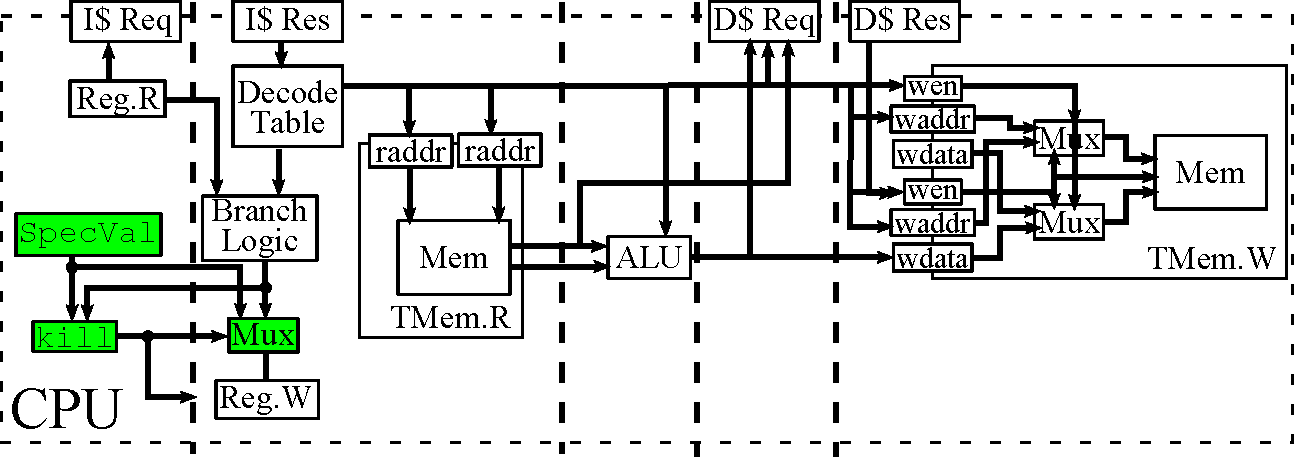
\includegraphics[width=\textwidth]{figures/pipelinespec.pdf}
  \caption{{\bf Speculation}. Using speculation to resolve hazards on
    the {\tt Reg} node whose read port is in the first stage and write port
  is in the second stage.}
  \label{fig:spec}
  \end{subfigure}
  \begin{subfigure}[t]{0.8\textwidth}
  \vspace{20pt}
  \centering
  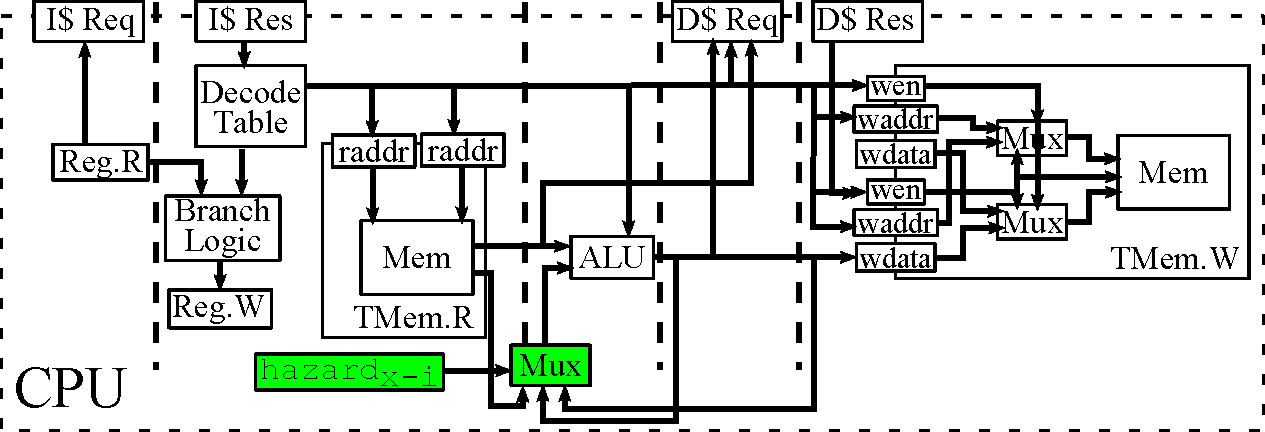
\includegraphics[width=\textwidth]{figures/pipelinebypass.pdf}
  \caption{{\bf Bypassing}. Bypassing network generated to forward ALU
  results from the third stage, fourth stage, and fifth stage to the
  {\tt TransactionalMem}'s second read port.}
  \label{fig:bypass}
  \end{subfigure}
\caption{Resolving hazards through speculation and bypassing.}
\label{fig:specbyp}
\end{figure*}

{\bf Interlocks}. The easiest way to resolve
hazards is through interlocks. This hazard resolution method requires
no additional input from the user. Every identified hazard is placed
into the stage of the read port that generates the hazard. In
Figure~\ref{fig:haz}, the hazards would be placed into the second
stage because the corresponding read port is in the second stage. We
then go through every stage and perform an {\tt OR} reduction on all
the hazards in that stage as well as all the hazard conditions in the
following stages to produce the stall condition for that stage. The
second part of interlocking a pipeline is to push bubbles. We go
through every stage and generate a {\tt pushBubble} signal if there is
a hazard condition in that stage and no following stages have a
hazard.

Figure~\ref{fig:int} shows the interlock logic that our tool
generates to handle the hazards from Figure~\ref{fig:haz}. Since
the {\tt TransactionalMem}'s read port is in the second stage, all the
{\tt hazard$_i$}s go into the second stage. When examining the second
stage, the tool would {\tt OR} reduce all the {\tt hazard}$_i$s to
generate a stall condition in the second stage. This stall condition
is used to stall the second and first stage. The same hazard
condition is then used to generate the {\tt pushBubble} signal. There
are no other sources of hazards further down the pipeline so the
hazard condition in the second stage is sufficient for pushing a
bubble into the second stage. Although not shown, we also generate
interlock logic for {\tt Reg} whose read port is in stage one and
write port is in stage two. We generate a hazard condition in the
first stage that is used to stall only the first stage. A bubble is
pushed into stage two if this hazard condition is asserted the second
stage's hazard condition is not asserted.

{\bf Speculation}. Our tool provides the function {\tt speculate} that
users can use to specify the stage element whose write value they want
to speculate along with the value they want to use for
speculation. This hazard resolution option is useful for transactions
that produce data that takes on one value with a very high likelihood
since we can have dependent transactions guess that value, allowing us
to avoid stalls. In a processor pipeline, for example, transactions
will usually write {\tt PC+4} to the PC register. To take advantage of
this regularity, we can guess that every transaction will write {\tt
  PC+4} to the {\tt PC} register. During elaboration, we modify the
Chisel graph to use the speculation value that the user provides to
update the node that the user marks for speculation. The speculation
value is pipelined until the actual data value is produced. We compare
the speculation value to the actual value. If the values match, we
continue as normal. Otherwise, we flush every stage starting at the
speculation stage up to but not including the stage where the
speculation value is checked.

To see how our speculation tool works, let's examine the pipeline in
Figure~\ref{fig:spec}. Notice that since every
transaction writes to the {\tt Reg} node in the second stage while
another transaction reads the node in the first stage, the interlock
hazard resolution option would cause our pipeline to stall every other
cycle. This scenario is a good match for the speculation resolution
option since transactions tend to write a very predictable value into
that node. We use the {\tt speculate} function to indicate that we
are guessing that the {\tt Reg} node will take on {\tt SpecVal}. We
mux in {\tt SpecVal} into the {\tt Reg} and then pipeline {\tt
  SpecVal} once (since the {\tt Reg} is read in the first stage and
written in the second stage). We compare {\tt SpecVal} to the actual
value to generate a kill signal that is asserted whenever the two
signals do not match. The kill signal is used to write the correct
value into the {\tt Reg} and we kill stage one.

{\bf Bypassing}. 
The user can use the {\tt bypassTo} function to annotate that a read port should be bypassed to by adding it to a list, which will be referred to as the bypass read ports list. The user may also use the {\tt avoidBypassFrom} function to annotate that certain write paths should never be bypassed from by adding the architectural state write ports associated with the write paths to be avoided to a list, which will be referred to as the non-bypass write ports list

In the graph transformation, for each read port added to bypass read ports
list, we look at all of the write ports not on the non-bypass write
ports list writing the architectural state the read port is attached
to and trace the write enable, write data, and write address signals
back through the pipeline. For each pipeline stage where the write
enable, write data, and write address are all available, we generate a mux in front of the original read port data wire that muxes in the write data from that pipeline stage on the condition {\tt wen \&\& waddr$_i$ === raddr}. We then remove that mux
condition from the list of interlock hazard conditions so that the
pipeline does not interlock when bypassing is possible. When a single write data path is available from multiple pipeline stages, the mux chain in front of the read port data sire is generated such that the write data from the earlier pipeline stage takes priority over the the write data from later pipeline stages, because data should be bypassed from the most recent transaction to go down the pipeline.

To see how our bypass logic generation works, let's examine the pipeline in Figure~\ref{fig:bypass}. In this example, the user annotated that the second read port of the TMem should be bypassed to and also annotated that the write path from the data cache should not be bypassed from. Assuming that the write enable and write address for the ALU is available starting from the 4th stage, our tool generates a mux chain to bypass from both the 4th stage and 5th stage version of the ALU output.
